\documentclass{article}
\usepackage{amsmath}
\usepackage{hyperref}
\usepackage{graphicx}
\usepackage{enumitem}

\begin{document}
The goal of this assignment is to build classifiers for the music genre dataset \href{https://www.kaggle.com/datasets/andradaolteanu/gtzan-dataset-music-genre-classification}{GTZAN} using different network architectures.
The dataset includes audio for 10 different music genres. Also, each audio has a visual representation constructed using MEL spectrograms.
Steps common to all architectures
\begin{enumerate}
    \item Resize the images to 224x224. This must be done when the images are loaded using torchvision.transforms.Resize. 
    \item Use PyTorch to randomly split the dataset into a training (80\%) and validation(20\%) datasets.
    \item Run the training for 50 epoch using Adam optimizer.
    \item For each of the architectures below plot the loss and accuracy vs epoch for both the training and validation datasets.
    \item For each of the architectures below plot the confusion matrix.
\end{enumerate}
The above tasks should be performed for each of the following architectures:
\begin{enumerate}[label=\Alph*]
    \item A fully connected network with two hidden layers\label{q:fc}.
    \item\label{q:conv} The convolutional network shown in figure \ref{fig:conv}
    \item Modify the CNN in figure \ref{fig:conv} by adding a batch normalization layer\label{q:bn}.
    \item Use three data augmentation methods on data and use it as an input to the architecture in part \ref{q:bn}\label{q:da}.
    
\end{enumerate} 
\begin{figure}[h]
    \begin{center}
        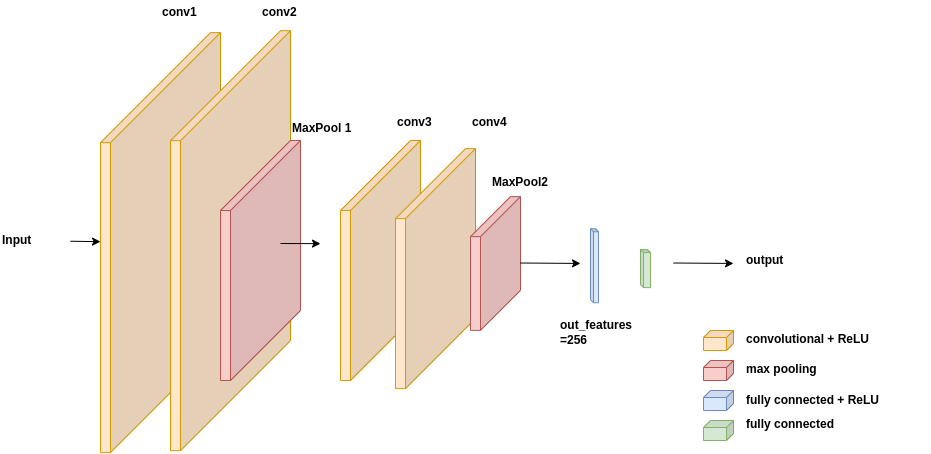
\includegraphics[width=0.9\textwidth]{course-work-conv.png}
    \end{center}
    \caption{Architecture used in part\ref{q:conv}\label{fig:conv}    }
\end{figure}
\section{Deliverables}
\begin{enumerate}
    \item A report of the results of parts \ref{q:fc}-\ref{q:conv}-\ref{q:bn}-\ref{q:da}, including plots of loss vs epoch, accuracy vs epoch, and confusion matrix for both training and validation sets.
    \item The report must include a discussion of MEL spectrograms with the appropriate references.
    \item Jupyter notebook for part \ref{q:da}
\end{enumerate}
\end{document}